\chapter{SCTP Agents}
\label{sec:sctpAgents}

   This chapter describes the SCTP agents developed for \ns~by the
   Protocol Engineering Lab at the University of Delaware.  The SCTP
   agents are all two-way agents, which means they are symmetric in the
   sense that they represent both a sender and receiver. However,
   bi-directional data has not yet been implemented. Each instance of an
   SCTP agent is either a sender or receiver.

   The SCTP agents are implemented in files matching the regular
   expression \nsf{\em{sctp/sctp*.\{cc, h\}}}.

   The SCTP agents currently supported are:

   \begin{itemize}\itemsep0pt

      \item Agent/SCTP - RFC2960 + draft-ietf-tsvwg-sctpimpguide-09.txt
       + draft-ietf-tsvwg-usctp-01.txt 

      \item Agent/SCTP/HbAfterRto - experimental extension (HEARTBEAT
      after RTO)

      \item Agent/SCTP/MultipleFastRtx - experimental extension (UD PEL's
      Multiple Fast Retransmit algorithm)

      \item Agent/SCTP/Timestamp - experimental extension (TIMESTAMP chunk)

      \item Agent/SCTP/MfrHbAfterRto - experimental extension that
      combines MultipleFastRtx and HbAfterRto

      \item Agent/SCTP/MfrTimestamp - experimental extension that
      combines MultipleFastRtx and Timestamp

   \end{itemize}

   Section~\ref{sec:baseSctp} provides a simple overview of the base SCTP
   agent with details of configuration parameters and
   commands. Section~\ref{sec:sctpExtensions} describes the SCTP
   extensions available. The details of the SCTP trace format used in
   packet trace files are explained in
   Section~\ref{sec:sctpTracing}. Section~\ref{sec:sctpApps} explains how
   to use legacy applications with SCTP and how to write SCTP-aware
   applications which exploit all SCTP's
   features. Section~\ref{sec:sctpExamples} provides examples scripts for
   both singled homed and multihomed endpoints.

   \section{The Base SCTP Agent}
   \label{sec:baseSctp}

      The base SCTP agent \code{Agent/SCTP} supports the features in the
      following sections of RFC2960, including modifications up to
      draft-ietf-tsvwg-sctpimpguide-13.txt.

      \begin{itemize}\itemsep0pt

	 \item[5.1] Normal Establishment of an Association (rudimentary
	 handshake)

	 \item[6.1] Transmission of DATA Chunks

	 \item[6.2] Acknowledgment on Reception of DATA Chunks

	 \item[6.3] Management Retransmission Timer

	 \item[6.4] Multihomed SCTP Endpoints

	 \item[6.5] Stream Identifier and Stream Sequence Number

	 \item[6.6] Ordered and Unordered Delivery 

	 \item[6.7] Report Gaps in Received DATA TSNs

	 \item[7.2] SCTP Slow-Start and Congestion Avoidance

	 \item[8.1] Endpoint Failure Detection

	 \item[8.2] Path Failure Detection

	 \item[8.3] Path Heartbeat (without upper layer control)

      \end{itemize}

      This agent also supports the Partial Reliability extension as of
      draft-ietf-tsvwg-usctp-01.txt.

      \paragraph{Association Establishment} The SCTP agent establishes an
      association using a four-way handshake, but the handshake is kept
      simple and does not strictly conform to RFC2960. The handshake does
      not exchange tags, and the INIT and COOKIE-ECHO chunks are not used
      to update the RTT.  Instead, RTT estimation begin with the first
      DATA chunk.

      \paragraph{Association Shutdown} Currently, the SCTP agent does not
      perform a proper shutdown. The association is abruptly terminated
      when the simulated connection ends. A shutdown procedure may be
      added in a future release.

      \paragraph{Multihoming} The underlying infrastructure of ns-2
      does not support multiple interfaces for a single node. To get
      around this limitation, our approach allows the general support for
      logically multihoming nodes that have a multihomed transport layer,
      such as SCTP. Each multihomed node is actually made up of more than
      one node. As shown in Figure~\ref{fig:multihomedNode}, a logically
      multihomed node is made up of a single "core node" and multiple
      "interface nodes", one for each simulated interface. The core node
      is connected to each interface node via a uni-directional link
      towards the interface node, but traffic never traverses these
      links. These links are only in place for the core node to make
      routing decisions. An SCTP agent simultaneously resides on all these
      nodes (i.e., the core and interface nodes), but actual traffic only
      goes to/from the interface nodes.  Whenever the SCTP agent needs to
      send data to a destination and does not know which outgoing
      interface to use, the agent firsts consults with the core node for a
      route lookup. Then, the SCTP agent performs the send from the
      appropriate interface node. Incoming data is received at one of the
      interface nodes directly and passed up to the SCTP agent. This
      solution is applicable to any transport protocol that requires
      multihoming functionality in ns-2. Note: the user must configure
      multihomed nodes using commands in Section~\ref{sec:sctpCommands}
      (an example is shown in Section~\ref{sec:multihomedExample}).

      \begin{figure}[tb] 
	\centerline{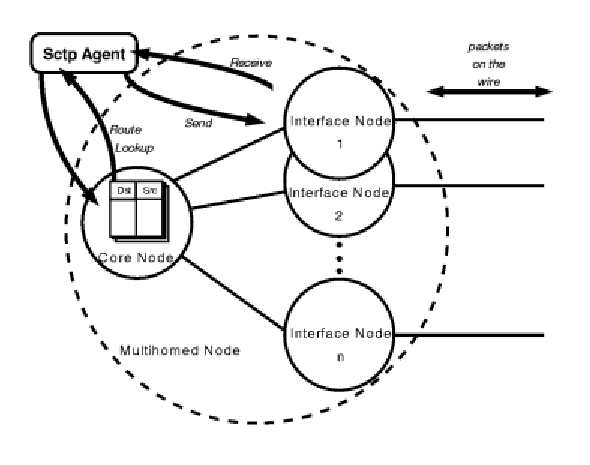
\includegraphics{sctp-multihomedNode}}
	\caption{Example of a Multihomed Node}
	\label{fig:multihomedNode} 
      \end{figure}

      \paragraph{Packet Number vs TSN Numbering} While \ns~starts numbering
      packets at 0, the SCTP module starts numbering DATA chunk TSNs at 1
      and assigns undefined TSN values (-1) to control chunks (ie, INIT,
      SACK, HEARTBEAT, etc). The four packets exchanged during the
      association establishment are counted in the packet enumeration, but
      do not show up in graphs. This information is important when doing
      things like specifying a drop list for the \code{ErrorModel}
      object. For example, packet 2 actually refers to the first SCTP
      packet with DATA chunk(s).


      \subsection{Configuration Parameters}
      \label{sec:sctpConfig}

	 SCTP supports several configuration variables which are TCL
	 bindable. Each of the variables described in this subsection is
	 both a class variable and an instance variable.  Changing the
	 class variable changes the default value for all agents that are
	 created subsequently.  Changing the instance variable of a
	 particular agent only affects the values used by that agent.  For
	 example,

	 \begin{program}
	 Agent/SCTP set pathMaxRetrans_ 5 \; Changes the class variable; 
	 $sctp set pathMaxRetrans_ 5 \; Changes pathMaxRetrans_ for the $sctp object only; 
         \end{program}

	 The default parameters for each SCTP agent are:

	 \begin{program}
	 Agent/SCTP set debugMask_ 0 \; 32-bit mask for modular toggle debugging control (see explanation);
	 Agent/SCTP set debugFileIndex_ -1 \; specifies debugging output file (see explanation);
	 Agent/SCTP set associationMaxRetrans_ 10\; RFC2960's Association.Max.Retrans;
	 Agent/SCTP set pathMaxRetrans_ 5 \; RFC2960's Path.Max.Retrans;
	 Agent/SCTP set changePrimaryThresh_ -1 \; change primary if error count exeeds thresh (default infinite);
	 Agent/SCTP set maxInitRetransmits_ 8 \; RFC2960's Max.Init.Retransmits;
	 Agent/SCTP set oneHeartbeatTimer_ 1 \; toggle HB timer for each dest vs one for all dests;
	 Agent/SCTP set heartbeatInterval_ 30 \; RFC2960's HB.interval in seconds;
	 Agent/SCTP set mtu_ 1500 \; MTU in bytes including IP header;
	 Agent/SCTP set initialRwnd_ 65536 \; initial receiver window in bytes (set on receiver side);
	 Agent/SCTP set initialSsthresh_ 65536 \; initial ssthresh value in bytes;
	 Agent/SCTP set initialCwnd_ 2 \; initial cwnd in multiple of (MTU - SCTP/IP headers);
	 Agent/SCTP set initialRto_ 3.0 \; default initial RTO = 3 secs;
	 Agent/SCTP set minRto_ 1.0    \; default min RTO = 1 sec;
	 Agent/SCTP set maxRto_ 60.0   \; default max RTO = 60 secs;
	 Agent/SCTP set fastRtxTrigger_ 4 \; 4 missing reports trigger fast rtx;
	 Agent/SCTP set numOutStreams_ 1 \; number of outgoing streams;
	 Agent/SCTP set numUnrelStreams_ 0 \; number of partially reliable streams (all grouped starting at stream 0);
	 Agent/SCTP set reliability_ 0 \; k-rtx value of all partially reliable streams;
	 Agent/SCTP set unordered_ 0 \; toggle all chunks are ordered/unordered;
	 Agent/SCTP set ipHeaderSize_ 20 \; IP header size;
	 Agent/SCTP set dataChunkSize_ 1468 \; includes data chunk header and restricted to 4 byte boundaries;
	 Agent/SCTP set useDelayedSacks_ 1 \; toggle on/off delayed sack algorithm (set on receiver side);
	 Agent/SCTP set sackDelay_ 0.200 \; rfc2960 recommends 200 ms;
	 Agent/SCTP set useMaxBurst_ 1 \; toggle on/off max burst;
	 Agent/SCTP set rtxToAlt_ 1 \; rtxs to which dest?  0 = same, 1 = alt, 2 = fast rtx to same + timeouts to alt;
	 Agent/SCTP set dormantAction_ 0 \; 0 = change dest, 1 = use primary, 2 = use last dest before dormant; 
	 Agent/SCTP set routeCalcDelay_ 0 \; time to calculate a route (see explanation);
	 Agent/SCTP set routeCacheLifetime_ 1.2 \; how long a route remains cached (see explanation);
	 Agent/SCTP set trace_all_ 0 \; toggle on/off print all variables on a trace event;
	 \end{program}

	 The \code{debugMask_} parameter is a 32-bit mask to turn on/off
	 debugging for particular functions. See
	 \nsf{\em{sctp/sctpDebug.h}} for the mappings of the bitmask. A -1
	 may be used to clear all bits, and 0 is used to turn off all
	 debugging. If \code{debug_} (the standard \ns~debug flag) is set to
	 1, then all the bits in \code{debugMask_} are set. Note: \ns~must
	 be compiled with \code{-DDEBUG} for this option to work.

	 The \code{debugFileIndex_} parameter is an integer to specify the
	 file used for debugging output by an SCTP agent. Each instance of
	 an SCTP agent can independently output debugging info to a
	 separate file. For example, the data sender can log debugging
	 output to one file, while the receiver logs to another file. If
	 \code{debugFileIndex_} is set to 0, the file used will be named
	 {\em debug.SctpAgent.0}. If -1 is used, the debug output is sent
	 to {\em stderr}. To avoid confusion, two SCTP agents should not
	 send debug output to the same file. The default is -1.  Note:
	 \ns~must be compiled with \code{-DDEBUG} for this option to work.

	 The configuration parameters that deal with ordering and
	 reliability options may be overridden by an SCTP-aware
	 application (see Section~\ref{sec:sctpApps}).

	 The \code{routeCalcDelay_} and \code{routeCacheLifetime_}
	 parameters are only used to optionally simulate overheads of
	 reactive routing protocols in MANETs without actually simulating
	 a MANET. (Do not use this feature if you are actually simulating
	 a MANET!) The default setting for \code{routeCalcDelay_} is 0
	 seconds, which means that this feature is turned off. The default
	 setting for \code{routeCacheLifetime_} is 1.2 seconds (ignored if
	 this feature is turned off), which is purposely set slightly
	 larger than the default min RTO to avoid a ``cache miss'' after a
	 single timeout event.

      \subsection{Commands}
      \label{sec:sctpCommands}

	 SCTP provides certain commands that can be used within TCL
	 scripts:

	 \paragraph{trace} Tracks given variables. The variable (and associated
	 information) is printed every time the value changes. Takes 1
	 argument:
	    \begin{itemize}

	       \item[] \code{cwnd_} Used to trace the cwnds of all
	       paths. 

	       \item[] \code{rto_} Used to trace the RTOs of all paths.

	       \item[] \code{errorCount_} Used to trace the error counters
	       of all paths.

	       \item[] \code{frCount_} Used to trace the number of times a
	       fast retransmit is invoked.

	       \item[] \code{mfrCount_} Used to trace the number of times
	       the multiple fast retransmit algorithm is invoked. This
	       trace variable can only be used with the MultipleFastRtx
	       extension agent. (See Section~\ref{ssec:mfr})

	       \item[] \code{timeoutCount_} Used to trace the total number of
	       times a timeout has occurred on all paths.

	       \item[] \code{rcdCount_} Used to trace the total number of
	       times a route calculation delay (see
	       Section~\ref{sec:sctpConfig}) has occurred on all paths.

	    \end{itemize}
	 Note: the actual value of these trace variables have no
	 meaning. They are simply used to trace corresponding variables
	 for potentially multihomed endpoints. For example, if a sender's
	 peer endpoint has two destinations, the sender will maintain two
	 cwnds. The \code{cwnd_} trace variable will trace both of these
	 cwnds together.

	 \paragraph{print} Provides the sampling method of tracing. This
	 command simply prints a given variable (and associated
	 information) per call.  Takes 1 argument: one of the trace
	 variables presented above.

	 \paragraph{set-multihome-core} Sets the core node for multihomed
	 endpoints. Takes 1 argument of type node. Mandatory for
	 multihomed endpoints and must not be set more than once per
	 endpoint.

	 \paragraph{multihome-add-interface} Adds an interface to a multihomed
	 endpoint. Takes 2 arguments of type node. Argument 1 is the core
	 node of the multihomed endpoint. Argument 2 is the interface node
	 to be added. Mandatory for multihomed endpoints. All interfaces
	 must be added after set-multihome-core is called and before
	 multihome-attach-agent is called.

	 \paragraph{multihome-attach-agent} Attaches an SCTP agent to a
	 multihomed endpoint. Takes 2 arguments. Argument 1 is the core
	 node. Argument 2 is the SCTP agent. Mandatory for multihomed
	 endpoints.

	 \paragraph{set-primary-destination} Sets the interface node of the peer
	 endpoint as the primary destination. Takes 1 argument of type
	 node. Optional and may be set more than once per endpoint. If not
	 used, a primary destination is chosen automatically.

	 \paragraph{force-source} Sets the interface node that packets will be
	 sent from. Takes 1 argument of type node. Optional and may be set
	 more than once per endpoint. If not used, routing will
	 automatically choose the source on a per packet basis.


   \section{Extensions}
   \label{sec:sctpExtensions}

      \subsection{HbAfterRto SCTP}

	 The HbAfterRto SCTP agent extends the current retransmission
	 policy. In addition to SCTP's current policy of retransmitting to
	 an alternate destination on a timeout, a heartbeat is sent
	 immediately to the destination on which a timeout occurred. Extra
	 heartbeats provide a mechanism for a sender to update an
	 alternate destination's RTT estimate more frequently, thus
	 resulting in a better RTT estimate on which to base the RTO
	 value.

	 For example, suppose a packet is lost in transit to the primary
	 destination, and later gets retransmitted to an alternate
	 destination. Also suppose that the retransmission times out. The
	 lost packet is retransmitted again to yet another alternate
	 destination (if one exists; otherwise, the primary). More
	 importantly, a heartbeat is also sent to the alternate
	 destination which timed out. If the heartbeat is successfully
	 acked, that destination acquires an additional RTT measurement to
	 help reduce its recently doubled RTO~\cite{SCTP_CARO_2003e}.

      \subsection{MultipleFastRtx SCTP}
      \label{ssec:mfr}

	 The MultipleFastRtx SCTP agent attempts to minimize the number of
	 timeouts which occur. Without the Multiple Fast Retransmit
	 algorithm, SCTP may only Fast Retransmit a TSN once. If a Fast
	 Retransmitted TSN is lost, a timeout is necessary to retransmit
	 the TSN again. The Multiple Fast Retransmit algorithm allows the
	 same TSN to be Fast Retransmitted several times if
	 needed. Without the Multiple Fast Retransmit algorithm, a large
	 window of outstanding data may generate enough SACKs to
	 incorrectly trigger more than one Fast Retransmit of the same TSN
	 in a single RTT.  To avoid these spurious Fast Retransmits, the
	 Multiple Fast Retransmit algorithm introduces a {\em
	 fastRtxRecover} state variable for each TSN Fast
	 Retransmitted. This variable stores the highest outstanding TSN
	 at the time a TSN is Fast Retransmitted. Then, only SACKs which
	 newly ack TSNs beyond {\em fastRtxRecover} can increment the
	 missing report for the Fast Retransmitted TSN. If the missing
	 report threshold for the Fast Retransmitted TSN is reached again,
	 the sender has enough evidence that this TSN was lost and can be
	 Fast Retransmitted again~\cite{SCTP_CARO_2003e}.

      \subsection{Timestamp SCTP}

	 The Timestamp SCTP agent introduces timestamps into each packet,
	 thus allowing a sender to disambiguate original transmissions
	 from retransmissions. By removing retransmission ambiguity,
	 Karn's algorithm can be eliminated, and successful
	 retransmissions on the alternate path can be used to update the
	 RTT estimate and keep the RTO value more accurate. With
	 timestamps, the sender has more samples for updating the RTT
	 estimate of alternate destination(s)~\cite{SCTP_CARO_2003e}.

      \subsection{MfrHbAfterRto SCTP}

         The MfrHbAfterRto SCTP agent combines the functionality of the
         HbAfterRto and MultipleFastRtx SCTP agents.


      \subsection{MfrHbAfterRto SCTP}

         The MfrTimestamp SCTP agent combines the functionality of the
         Timestamp and MultipleFastRtx SCTP agents.

   \section{Tracing SCTP Dynamics}
   \label{sec:sctpTracing}

      SCTP packets generated by one of the SCTP agents and destined for a
      peer SCTP agent over a traced link (see section~\ref{chap:trace})
      will generate a trace file with lines of the form:

      \begin{verbatim}
      + 0.5 1 4 sctp 56 -------I 0 1.0 4.0 1 -1 4 65535 65535
      - 0.5 1 4 sctp 56 -------I 0 1.0 4.0 1 -1 4 65535 65535
      r 0.700896 1 4 sctp 56 -------I 0 1.0 4.0 1 -1 4 65535 65535
      + 0.700896 4 1 sctp 56 -------I 0 4.0 1.0 1 -1 5 65535 65535
      - 0.700896 4 1 sctp 56 -------I 0 4.0 1.0 1 -1 5 65535 65535
      r 0.901792 4 1 sctp 56 -------I 0 4.0 1.0 1 -1 5 65535 65535
      + 0.901792 1 4 sctp 36 -------I 0 1.0 4.0 1 -1 6 65535 65535
      - 0.901792 1 4 sctp 36 -------I 0 1.0 4.0 1 -1 6 65535 65535
      r 1.102368 1 4 sctp 36 -------I 0 1.0 4.0 1 -1 6 65535 65535
      + 1.102368 4 1 sctp 36 -------I 0 4.0 1.0 1 -1 7 65535 65535
      - 1.102368 4 1 sctp 36 -------I 0 4.0 1.0 1 -1 7 65535 65535
      r 1.302944 4 1 sctp 36 -------I 0 4.0 1.0 1 -1 7 65535 65535
      + 1.302944 1 4 sctp 1500 -------D 0 1.0 4.0 1 1 8 0 0
      - 1.302944 1 4 sctp 1500 -------D 0 1.0 4.0 1 1 8 0 0
      + 1.302944 1 4 sctp 1500 -------D 0 1.0 4.0 1 2 9 0 1
      - 1.326624 1 4 sctp 1500 -------D 0 1.0 4.0 1 2 9 0 1
      r 1.526624 1 4 sctp 1500 -------D 0 1.0 4.0 1 1 8 0 0
      r 1.550304 1 4 sctp 1500 -------D 0 1.0 4.0 1 2 9 0 1
      + 1.550304 4 1 sctp 48 -------S 0 4.0 1.0 1 2 11 65535 65535
      - 1.550304 4 1 sctp 48 -------S 0 4.0 1.0 1 2 11 65535 65535
      r 1.751072 4 1 sctp 48 -------S 0 4.0 1.0 1 2 11 65535 65535
      ...
      + 19.302944 4 1 sctp 56 -------H 0 2.0 5.0 1 -1 336 65535 65535
      - 19.302944 4 1 sctp 56 -------H 0 2.0 5.0 1 -1 336 65535 65535
      r 19.303264 4 1 sctp 56 -------H 0 4.0 1.0 1 -1 322 65535 65535
      + 19.303264 1 4 sctp 56 -------B 0 1.0 4.0 1 -1 337 65535 65535
      - 19.327584 1 4 sctp 56 -------B 0 1.0 4.0 1 -1 337 65535 65535
      r 19.52848 1 4 sctp 56 -------B 0 1.0 4.0 1 -1 337 65535 65535
      \end{verbatim}

      When tracing SCTP, packets of type {\sf sctp} are relevant.  Their
      packet type, chunk type, packet size, TSN (CumAck point for SACK
      chunks), stream ID, SSN, and arrival/depart/drop time are given by
      field positions 5, 7 (flag position 8), 6, 12, 14, 15, and 2,
      respectively. If a packet has more than one chunk, a line is printed
      for each chunk. A future release should include a field to indicate
      which chunk of the packet a line refers to (e.g., 2:3 could identify
      the 2nd chunk of a packet which contains 3 chunks). Since control
      chunks do not use TSNs, stream IDs, or SSNs, the trace lines for
      these chunks use undefined numbers (-1 or 65535) for these fields.
      The {\sf +} indicates a packet arrival, {\sf d} a drop, and {\sf -}
      a departure.

      Flag position 8 of field 7 indicate the chunk type as follows. The
      {\sf I} flag indicates an association initiation control chunk
      (INIT, INIT-ACK, COOKIE-ECHO, COOKIE-ACK). A future release should
      use {\sf I} for the INIT and INIT-ACK chunks, and {\sf C} for the
      COOKIE-ECHO and COOKIE-ACK chunks. The {\sf D}, {\sf S}, {\sf H},
      and {\sf B} flags indicate a DATA chunk, a SACK, a HEARTBEAT chunk,
      and a HEARTBEAT-ACK chunk.

      A number of scripts process this file to produce graphical output or
      statistical summaries (for example, see the {\tt finish} procedure
      in \nsf{\em{tcl/test/test-suite-sctp.tcl}}).

   \section{SCTP Applications}
   \label{sec:sctpApps}

      SCTP supports legacy \ns~applications, but they obviously cannot
      completely exploit all SCTP's features. For these applications, the
      TCL-bound SCTP configuration parameters can be used to set
      reliability and ordering options. However, these options cannot be
      controlled per message using these parameters. Only SCTP-aware
      application can be written to do so. \ns~applications wishing to
      become SCTP-aware can use the sendmsg API as follows (see
      \nsf{\em{apps/sctp\_app1.\{cc, h\}}} as an example).

      \begin{enumerate}

	 \item Create and fill an instance of the \code{AppData_S}
	 structure (see \nsf{\em{sctp/sctp.h}}). The \code{AppData_S}
	 structure has the following fields:

	 \begin{itemize}

	    \item[] \code{usNumStreams} is the number of outgoing streams
	    to setup during negotiation. Although this field is passed
	    with every sendmsg call, it is only used during association
	    setup. Once the association is established, this field is
	    ignored.

	    \item[] \code{usNumUnreliable} is the number of outgoing
	    streams which are unreliable (now called partially
	    reliable). The sender simply sets the lowest outgoing stream
	    to unreliable/partially-reliable; the remaining ones are
	    reliable. This field is also only used during association
	    establishment.

	    \item[] \code{usStreamId} is the stream ID of a message.

	    \item[] \code{usReliability} is the reliability level (k-rtx
	    value) of a message. This field is ignored if the message is
	    sent on a reliable stream.

	    \item[] \code{eUnordered} is the unordered boolean flag for a
	    message.

	    \item[] \code{uiNumBytes} is the number of bytes in a message.

	 \end{itemize}

	 \item Pass this object as the second parameter in SCTP's sendmsg:

	 \code{sctpAgent->sendmsg(numBytes, (char *)appData);}

      \end{enumerate}

   \section{Example Scripts}
   \label{sec:sctpExamples}

      \subsection{Singled Homed Example}

	 \begin{program}
	 Trace set show_sctphdr_ 1 \; this needs to be set for tracing SCTP packets;

	 set ns [new Simulator]
	 set allchan [open all.tr w]
	 $ns trace-all $allchan

	 proc finish {} \{
	    exit 0
	 \}

	 set n0 [$ns node]
	 set n1 [$ns node]
	 $ns duplex-link $n0 $n1 .5Mb 200ms DropTail

	 # NOTE: The debug files (in this example, they would be debug.SctpAgent.0
	 #       and debug.SctpAgent.1) contain a lot of useful info. They can be 
	 #       used to trace every packet sent, received, and processed.
	 #
	 set sctp0 [new Agent/SCTP]
	 $ns attach-agent $n0 $sctp0
	 $sctp0 set debugMask_ 0x00303000 \; refer to sctpDebug.h for mask mappings;
	 $sctp0 set debugFileIndex_ 0

	 set trace_ch [open trace.sctp w]
	 $sctp0 set trace_all_ 0 \; do not trace all variables on one line;
	 $sctp0 trace cwnd_      \; trace cwnd for all destinations;
	 $sctp0 attach $trace_ch

	 set sctp1 [new Agent/SCTP]
	 $ns attach-agent $n1 $sctp1
	 $sctp1 set debugMask_ -1         \; use -1 to turn on all debugging;
	 $sctp1 set debugFileIndex_ 1

	 $ns connect $sctp0 $sctp1

	 set ftp0 [new Application/FTP]
	 $ftp0 attach-agent $sctp0

	 $ns at 0.5 "$ftp0 start"
	 $ns at 4.5 "$ftp0 stop"
	 $ns at 5.0 "finish"

	 $ns run
	 \end{program}


      \subsection{Multihomed Example}
      \label{sec:multihomedExample}

	 \begin{verbatim}
	 # This example demonstrates multihoming. Two SCTP endpoints, each
	 # with 2 interfaces, are directly connected between each pair of
	 # interfaces.  In the middle of the association, a change primary
	 # is done. Running nam helps to visualize the multihomed
	 # architecture.
	 #
	 #       host0_if0      O===========O    host1_if0
	 #                     /             \
	 #       host0_core   O               O  host1_core
	 #                     \             /
	 #       host0_if1      O===========O    host1_if1
	 \end{verbatim}
	 \begin{program}
	 Trace set show_sctphdr_ 1

	 set ns [new Simulator]
	 set nf [open sctp.nam w]
	 $ns namtrace-all $nf
	 set allchan [open all.tr w]
	 $ns trace-all $allchan

	 proc finish {} \{
	    exec nam sctp.nam &
	    exit 0
	 \}

	 set host0_core [$ns node]
	 set host0_if0 [$ns node]
	 set host0_if1 [$ns node]
	 $host0_core color Red
	 $host0_if0 color Red
	 $host0_if1 color Red
	 $ns multihome-add-interface $host0_core $host0_if0
	 $ns multihome-add-interface $host0_core $host0_if1

	 set host1_core [$ns node]
	 set host1_if0 [$ns node]
	 set host1_if1 [$ns node]
	 $host1_core color Blue
	 $host1_if0 color Blue
	 $host1_if1 color Blue
	 $ns multihome-add-interface $host1_core $host1_if0
	 $ns multihome-add-interface $host1_core $host1_if1

	 $ns duplex-link $host0_if0 $host1_if0 .5Mb 200ms DropTail
	 $ns duplex-link $host0_if1 $host1_if1 .5Mb 200ms DropTail

	 set sctp0 [new Agent/SCTP]
	 $ns multihome-attach-agent $host0_core $sctp0

	 set trace_ch [open trace.sctp w]
	 $sctp0 set trace_all_ 1           \; print all on a single trace event;
	 $sctp0 trace rto_
	 $sctp0 trace errorCount_
	 $sctp0 attach $trace_ch

	 set sctp1 [new Agent/SCTP]
	 $ns multihome-attach-agent $host1_core $sctp1

	 $ns connect $sctp0 $sctp1

	 set ftp0 [new Application/FTP]
	 $ftp0 attach-agent $sctp0

	 $sctp0 set-primary-destination $host1_if0 \; set primary before association starts;

	 $ns at 7.5 "$sctp0 set-primary-destination $host1_if1" \; change primary;
	 $ns at 7.5 "$sctp0 print cwnd_" \; print all dests' cwnds at time 7.5;

	 $ns at 0.5 "$ftp0 start"
	 $ns at 9.5 "$ftp0 stop"
	 $ns at 10.0 "finish"

	 $ns run
	 \end{program}

\endinput
